\chapter{Results of Optical Design} % Main chapter title
\noindent\textbf{\large Contents:}

\noindent\hrulefill
\noindent\startcontents[chapters]
\noindent\printcontents[chapters]{}{1}{}
\noindent\hrulefill
\label{Chapter4}

\section{Spot Size}
\label{sec:spot_result}

One of the requirements of an AO system is to be diffraction limited.  One prerequisite 
is for the spot size to be smaller than the Airy Disk of the system.  ZEMAX is
able to display the Airy disk on spot diagrams.  Since the system could not analyze
a spot array, this section will look at the results from a single lens and then that
of the lenslet array.

\subsection{Single lens}
\label{sec:single_spot}

Here, a single lens over the whole aperture was used in place of an MLA.  This
allowed for the system to optimize with a known spot size and allowing all of the
rays that pass through the entrance pupil to converge in the image plane.  A f/10
lens was put in place as a scale up of the lenslet.  As the system optimized,
eventually the spot size became smaller than the Airy Disk of the system, thus
becoming diffraction limited.  

\begin{figure}[h!]
\centering
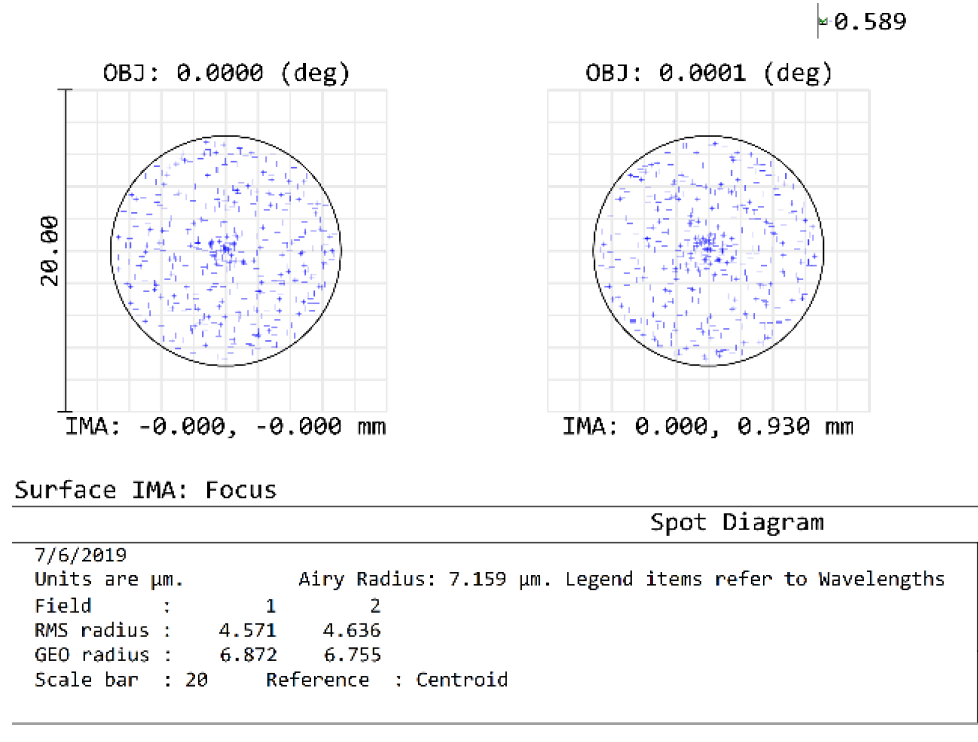
\includegraphics[width=14 cm]{Figures/spot_size_lens.png}
\caption{A figure of both fields having the spots within the Airy Disk.}
\label{fig:spot_lens}
\end{figure}

As seen in Figure \ref{fig:spot_lens}, the Airy disk has a radius of $7.159 \mu m$,
while the spot has an RMS radius of $4.571 \mu m$.  While the spot size could be
improved, the wavefront error started to degrade as spot size decreased.  Since we 
are only imaging spots and not looking for definition, this should still prove to 
perform just as well.

\subsection{Lenslet Array}
\label{sec:lenslet_result}

As described in Section \ref{sec:Optical_real}, the lenslet array was designed based
off hand calculations and focused by hand.  The system did not go through an
optimization process.  So it is crucial to understand if the system is performing
adequately. First, since the aperture size of the lenslet changed, so did too the
radius of the Airy Disk.  Only spots off-axis could be analyzed due to light being
blocked by M2.

% \begin{figure}[h!]
% \centering
% 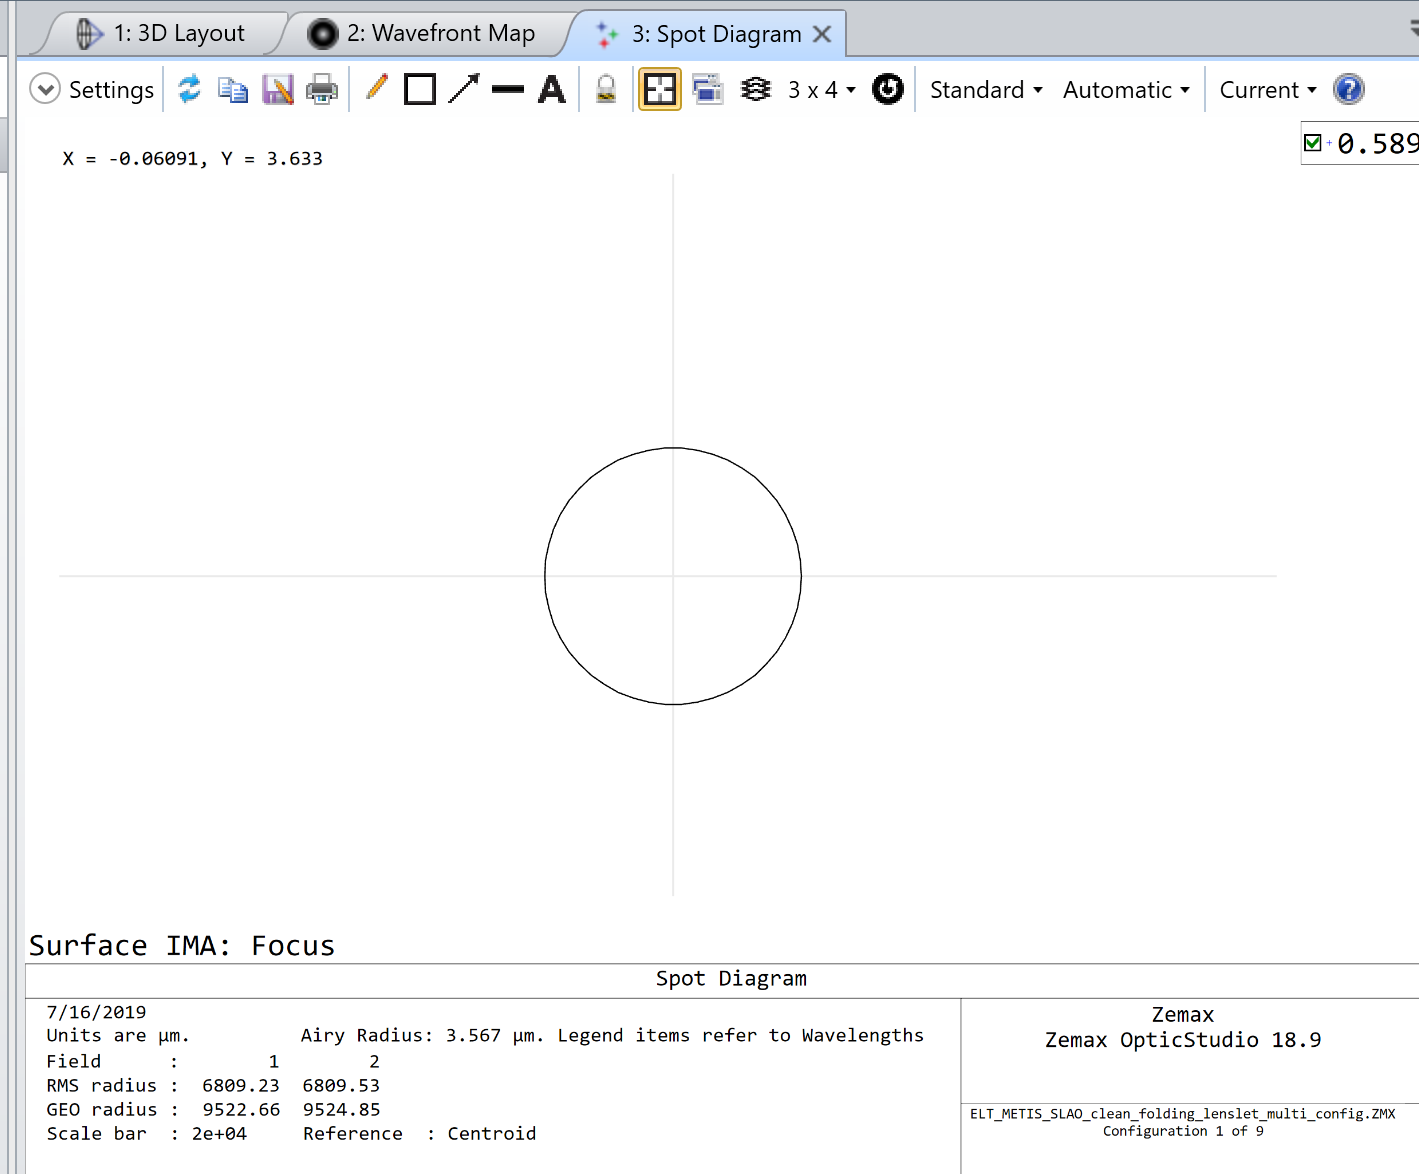
\includegraphics[width=14 cm]{Figures/Results/lenslet_airy_disk.png}
% \caption{Here you can see that the Airy disk radius is now $3.567 \mu m$.  There is no spot inside the Airy disk due to no light passing through M2 of ELT.}
% \label{fig:MLA_Airy}
% \end{figure}

\begin{figure}[h!]
\centering
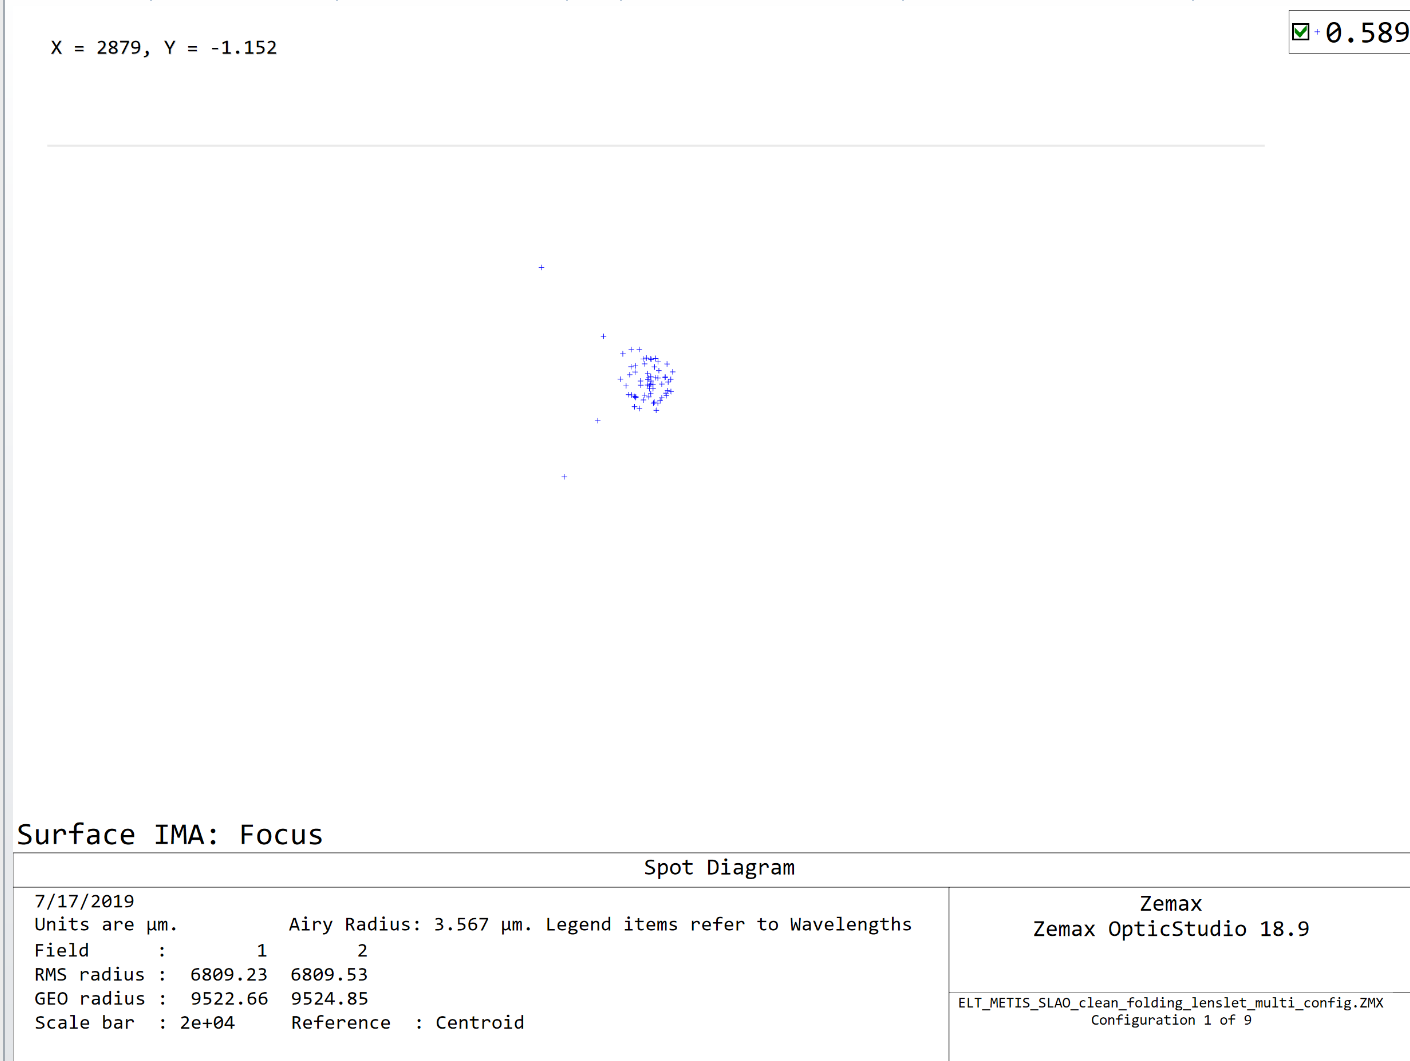
\includegraphics[width=10 cm]{Figures/Results/on_axis_top.png}
\caption{A Figure with the calculated Airy Disk radius in the data sheet on the bottom left.  The coordinates in the top left are displayed in microns.  It should be noted that there is some aberration effect taking place.}
\label{fig:spot_lenslet}
\end{figure}

When the lenslet array is substituted in, the Airy disk now has a radius of $3.567
\mu m$. While it may not be the most scientific way, the next step is to look at the
spot and determine its diameter based off of the coordinate positions of the cursor.
When the cursor was moved from the top of the spot to the bottom, the cursor changed
roughly $0.5 \mu m$.  That is a radius of $0.25 \mu m$.  This means that the spot
size is roughly an order of magnitude smaller that the calculated Airy disk by ZEMAX.

\begin{figure}[h!]
\centering
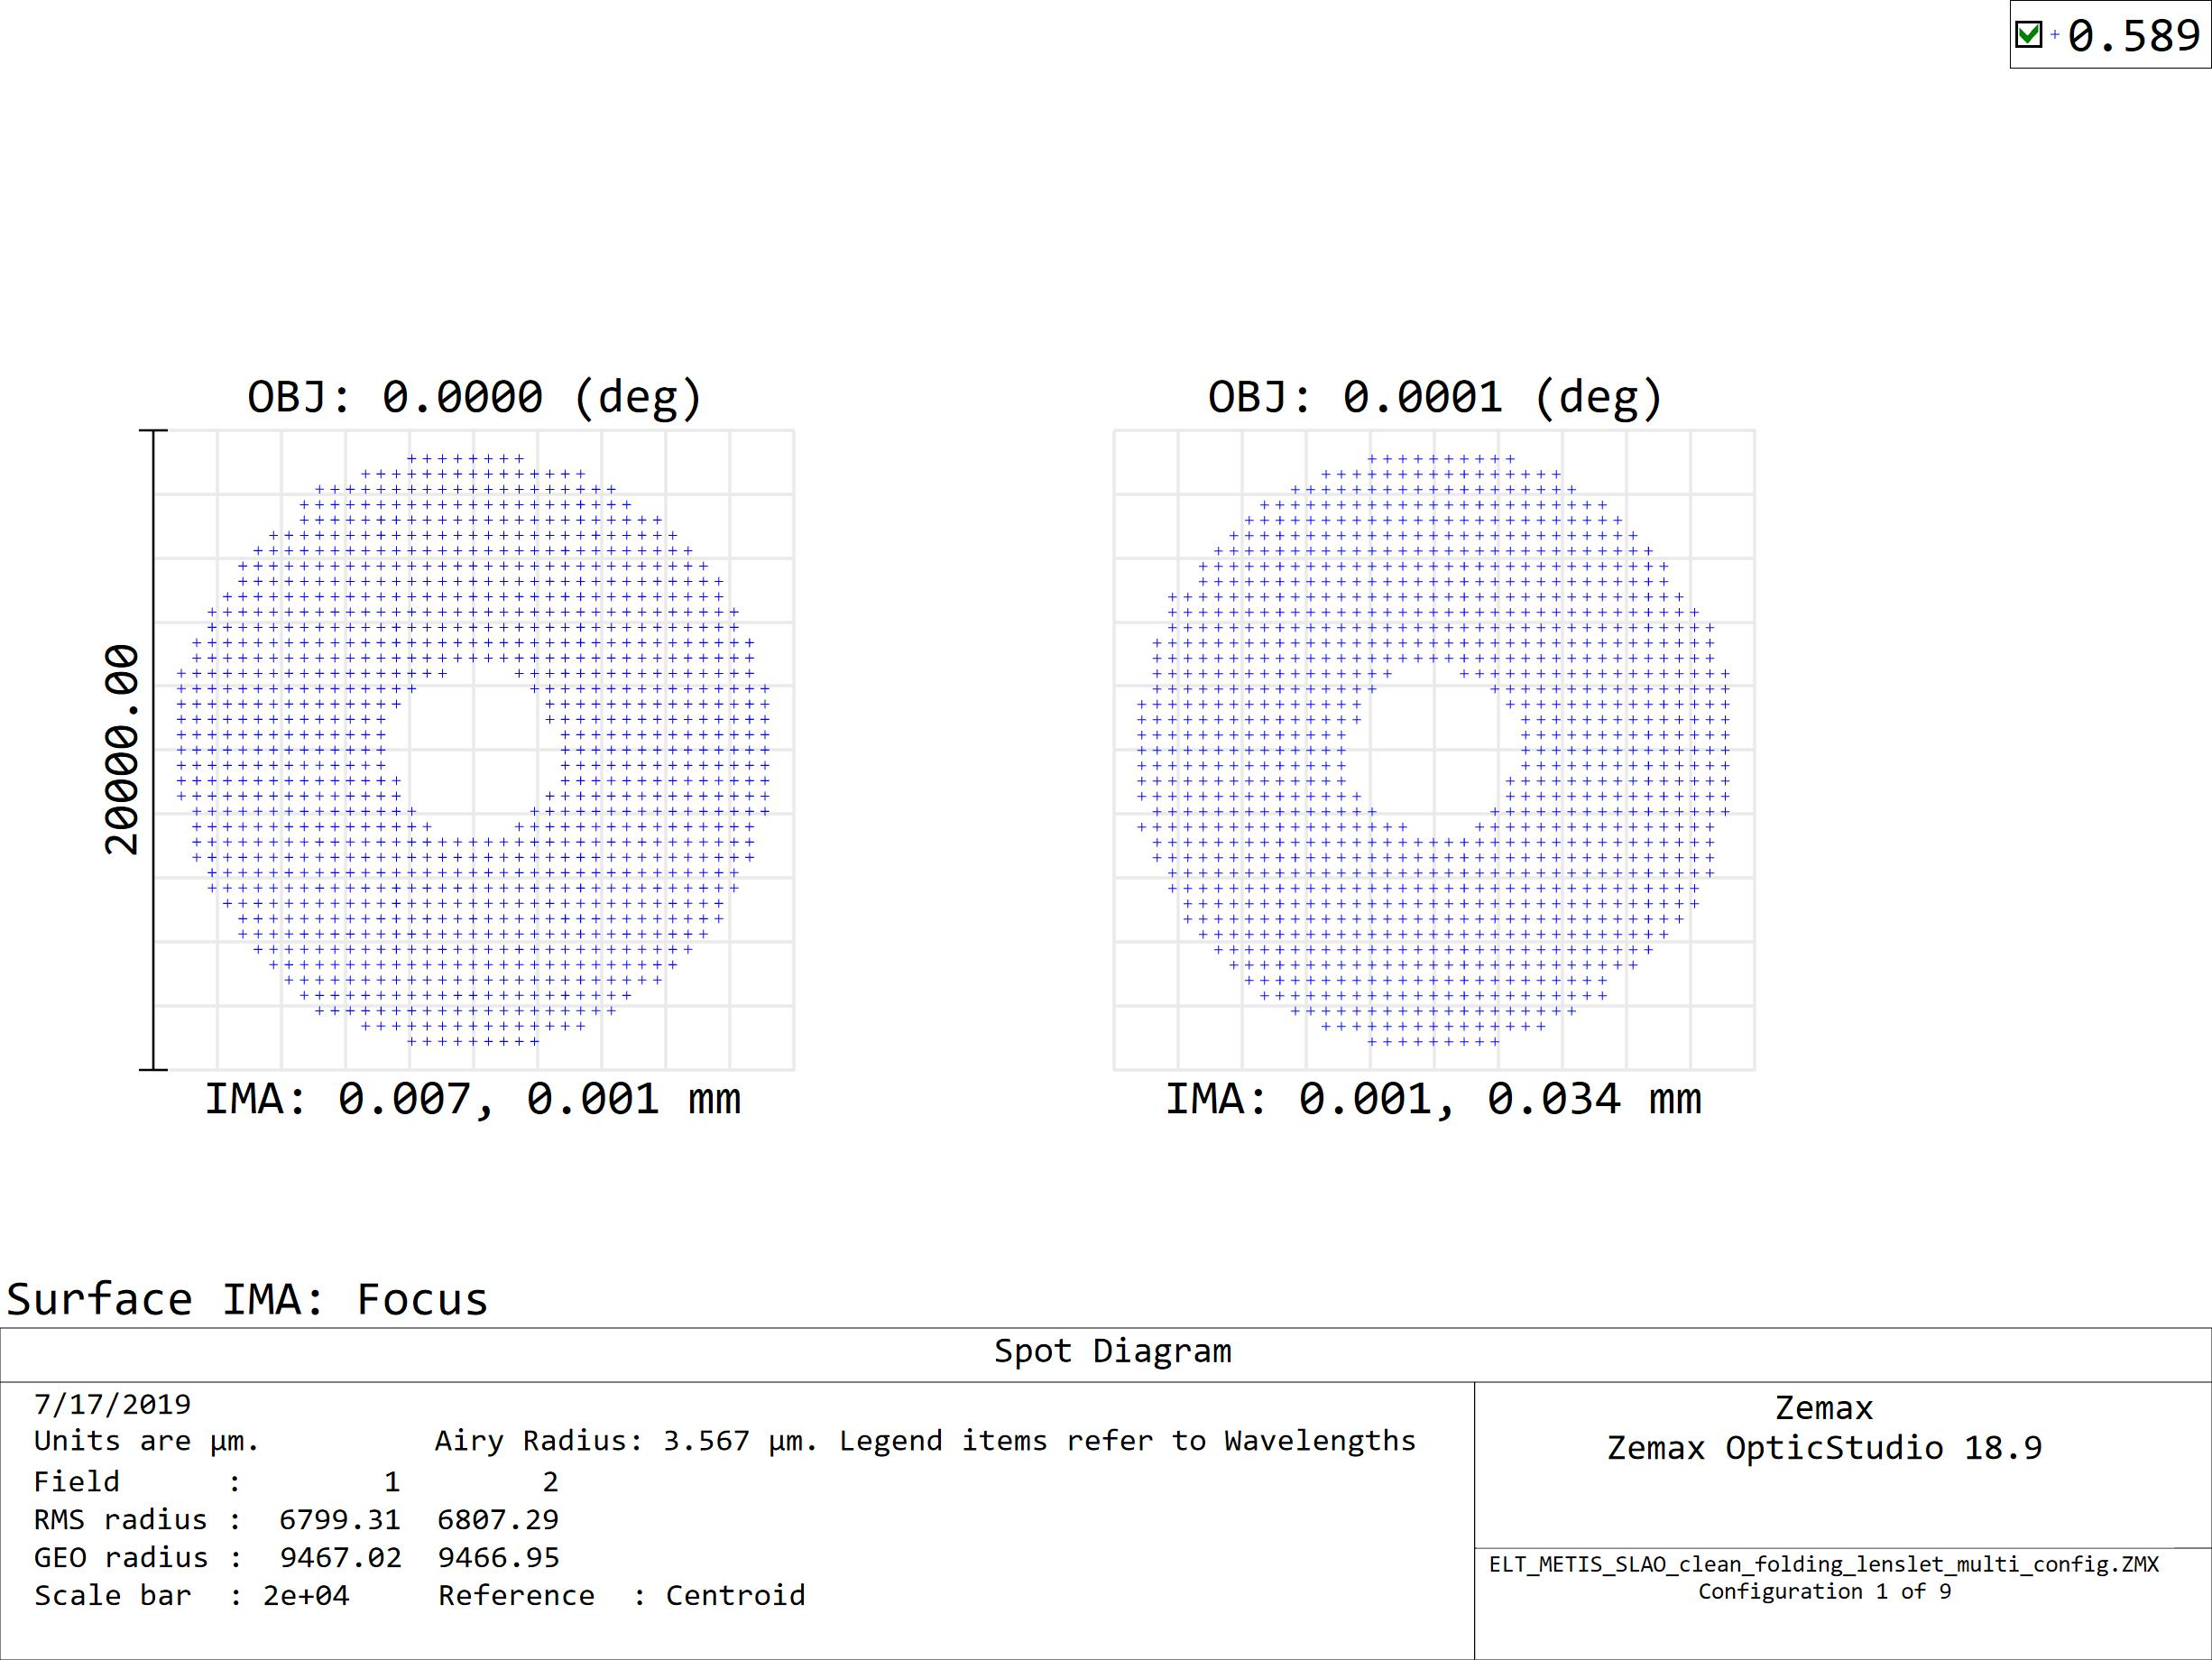
\includegraphics[width=14 cm]{Figures/Results/MLA_SpotDiagram.jpg}
\caption{Here a side by side comparison of two different field angles and their spots.  Obviously the spots are too small to see anything revealing.}
\label{fig:lenslet_spot_array}
\end{figure}

The full array of spots is 19.6mm across.  So side by side comparisons of the fully 
array do not show anything particularly revealing.  However, it does give a good
idea what the system will see while in use (Figure \ref{fig:lenslet_spot_array}).

\subsection{Spot Elongation}
\label{sec:spot_elong}

All of the ELT's lasers are mounted on the perimeter of the telescope support
structure.  There is no center mounted laser (usually behind M2).  This means that
the system will suffer from spot elongation even when pointing at zenith (Figure 
\ref{fig:spot_elong}).  Since the Sodium layer in the Earth's atmosphere has an
approximate thickness of 10 km, there will be illumination all along that thickness.
We made the assumption that the laser spot would be pointed to directly above the
telescope.  Therefore, we assumed that the on-axis portion of the laser was in the
center of the Sodium Layer. How this was handled in ZEMAX was to find the off-axis
angle for the min and max altitude of the spot at each zenith angle.  Each of these
were a separate configuration in ZEMAX.

\begin{figure}[h!]
\centering
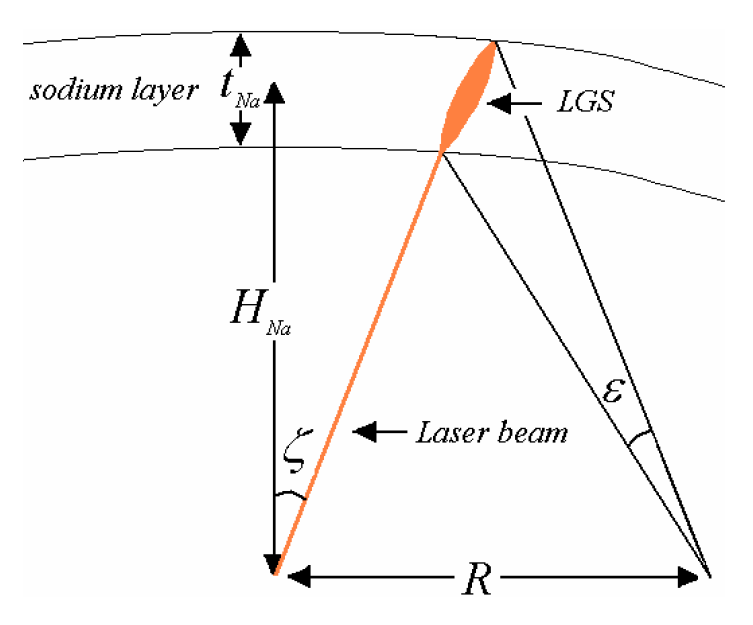
\includegraphics[width=8 cm]{Figures/Results/spot_elongation.png}
\caption{A figure showing an example of what causes spot \\elongation \cite{sodium}}
\label{fig:spot_elong}
\end{figure}

From these configurations, it is apparent that there is the greatest amount of spot
elongation when pointing at zenith.  Need to talk about this more after getting
images.

\begin{figure}[h!]
\centering
\includegraphics[width=8 cm]{Figures/Results/Image_in_process.png}
\caption{A Figure showing the spot size... Coming soon.  Waiting on Patrick}
\label{fig:spot_array_elong}
\end{figure}


It should also be noted that Figure \ref{fig:spot_array_elong} was evaluated with
the annular mirror having a central obscuration (Diameter= 42.9mm \cite{arcier}) in
it to simulate the hole in the mirror.  There does not appear to be any light lost
from this feature from spot elongation.


\section{Wavefront Map}
\label{sec:wave_map}

In the 2016 status update of METIS, it was stated that there should be a maximum
RMS wavefront error shall be less than 100nm \cite{METISSPIE2016}.  ZEMAX outputs
a wavefront map in units of waves.  Since the light coming from the laser spot is
589nm.  The RMS should be:

\begin{equation}
    \frac{100nm}{589nm} = 0.17 waves
\end{equation}

\begin{figure}[h!]
\centering
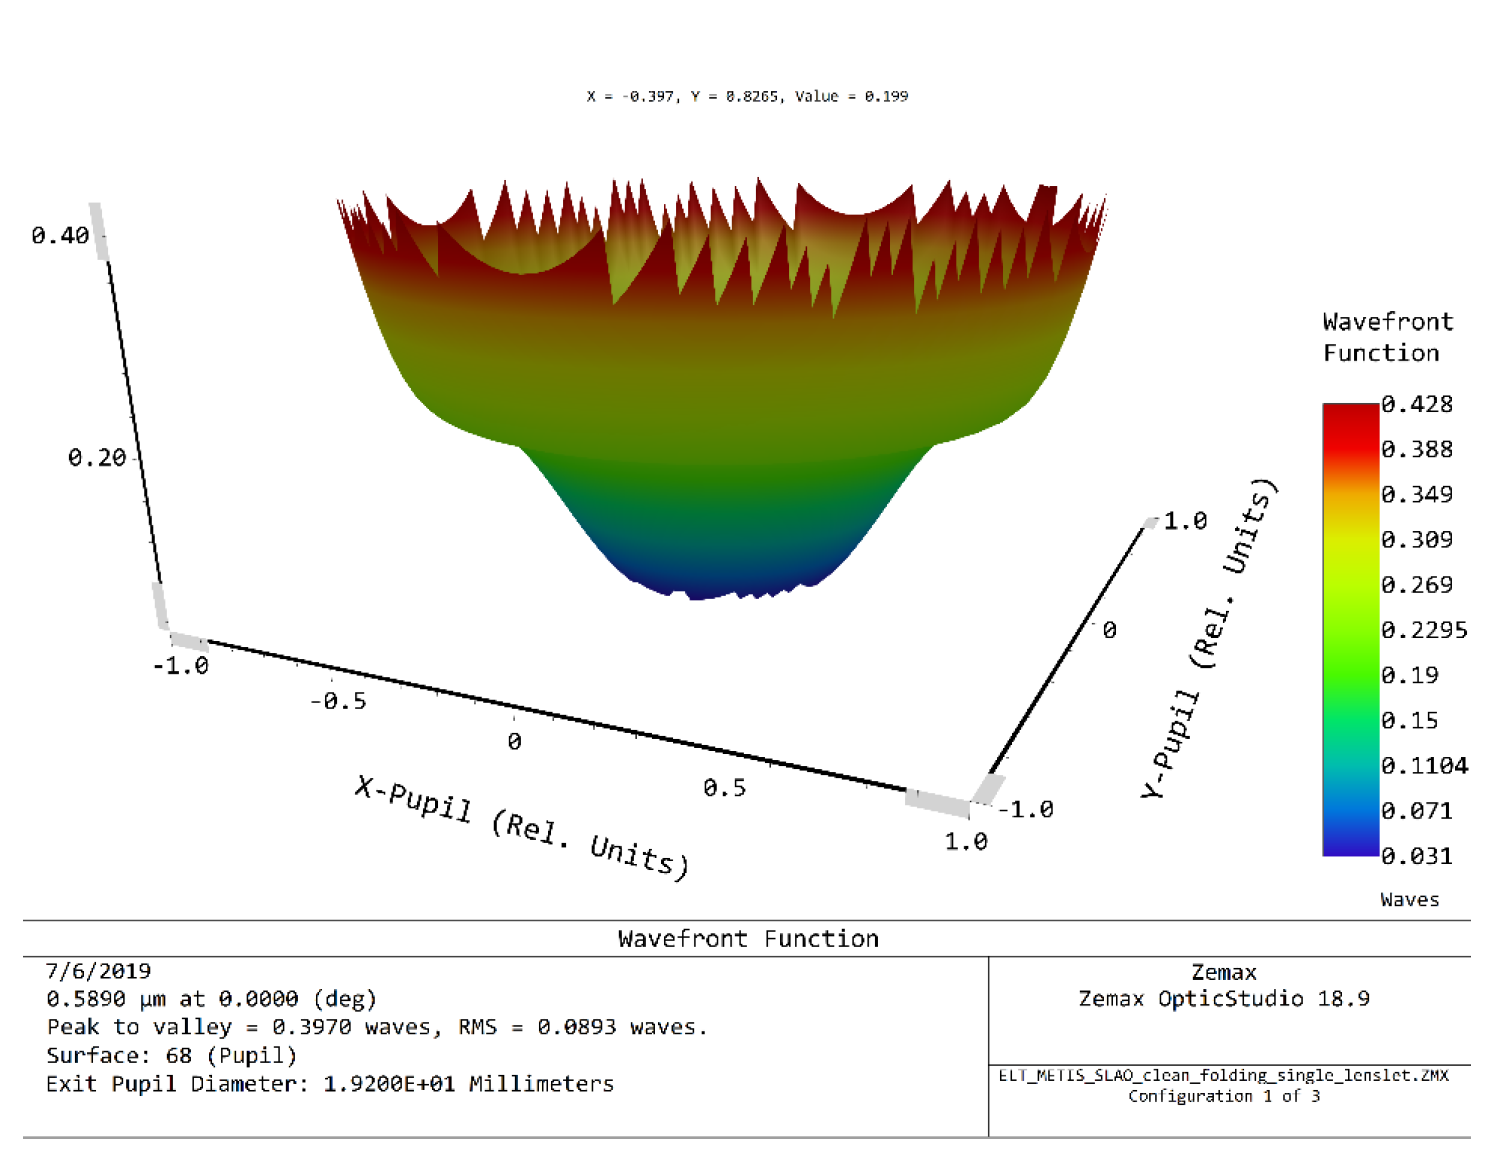
\includegraphics[width=14 cm]{Figures/Results/wavefront.png}
\caption{Here is a map of the wavefront at the lenslet array.  PTV = 0.397 ; RMS = 0.0893 waves.}
\label{fig:wavefront}
\end{figure}

In Figure \ref{fig:wavefront}, we can see that the on axis performance is almost a 
factor of 2 better than the requirement.  For a full list of wavefront
characteristics, see Appendix \ref{AppendixA}.

\section{Aspherical Component}
\label{sec:asphere}

One of the main purposes of this research was to look into ways to avoid aspherical
surfaces.  However, having one asphere can make a design cheaper in the end.  It is
important however to have a manufacturable asphere.  In general, the more material
that needs to be removed, the more expensive the part.  The amount of material needed to be removed for this aspherical component is all fractions of a millimeter
and over an aperture size of 20 mm.  Upon inspection, the map appears close to a
parabolic shape.  All of these are good factors for manufacturing an aspherical
component.

\begin{figure}[h!]
\centering
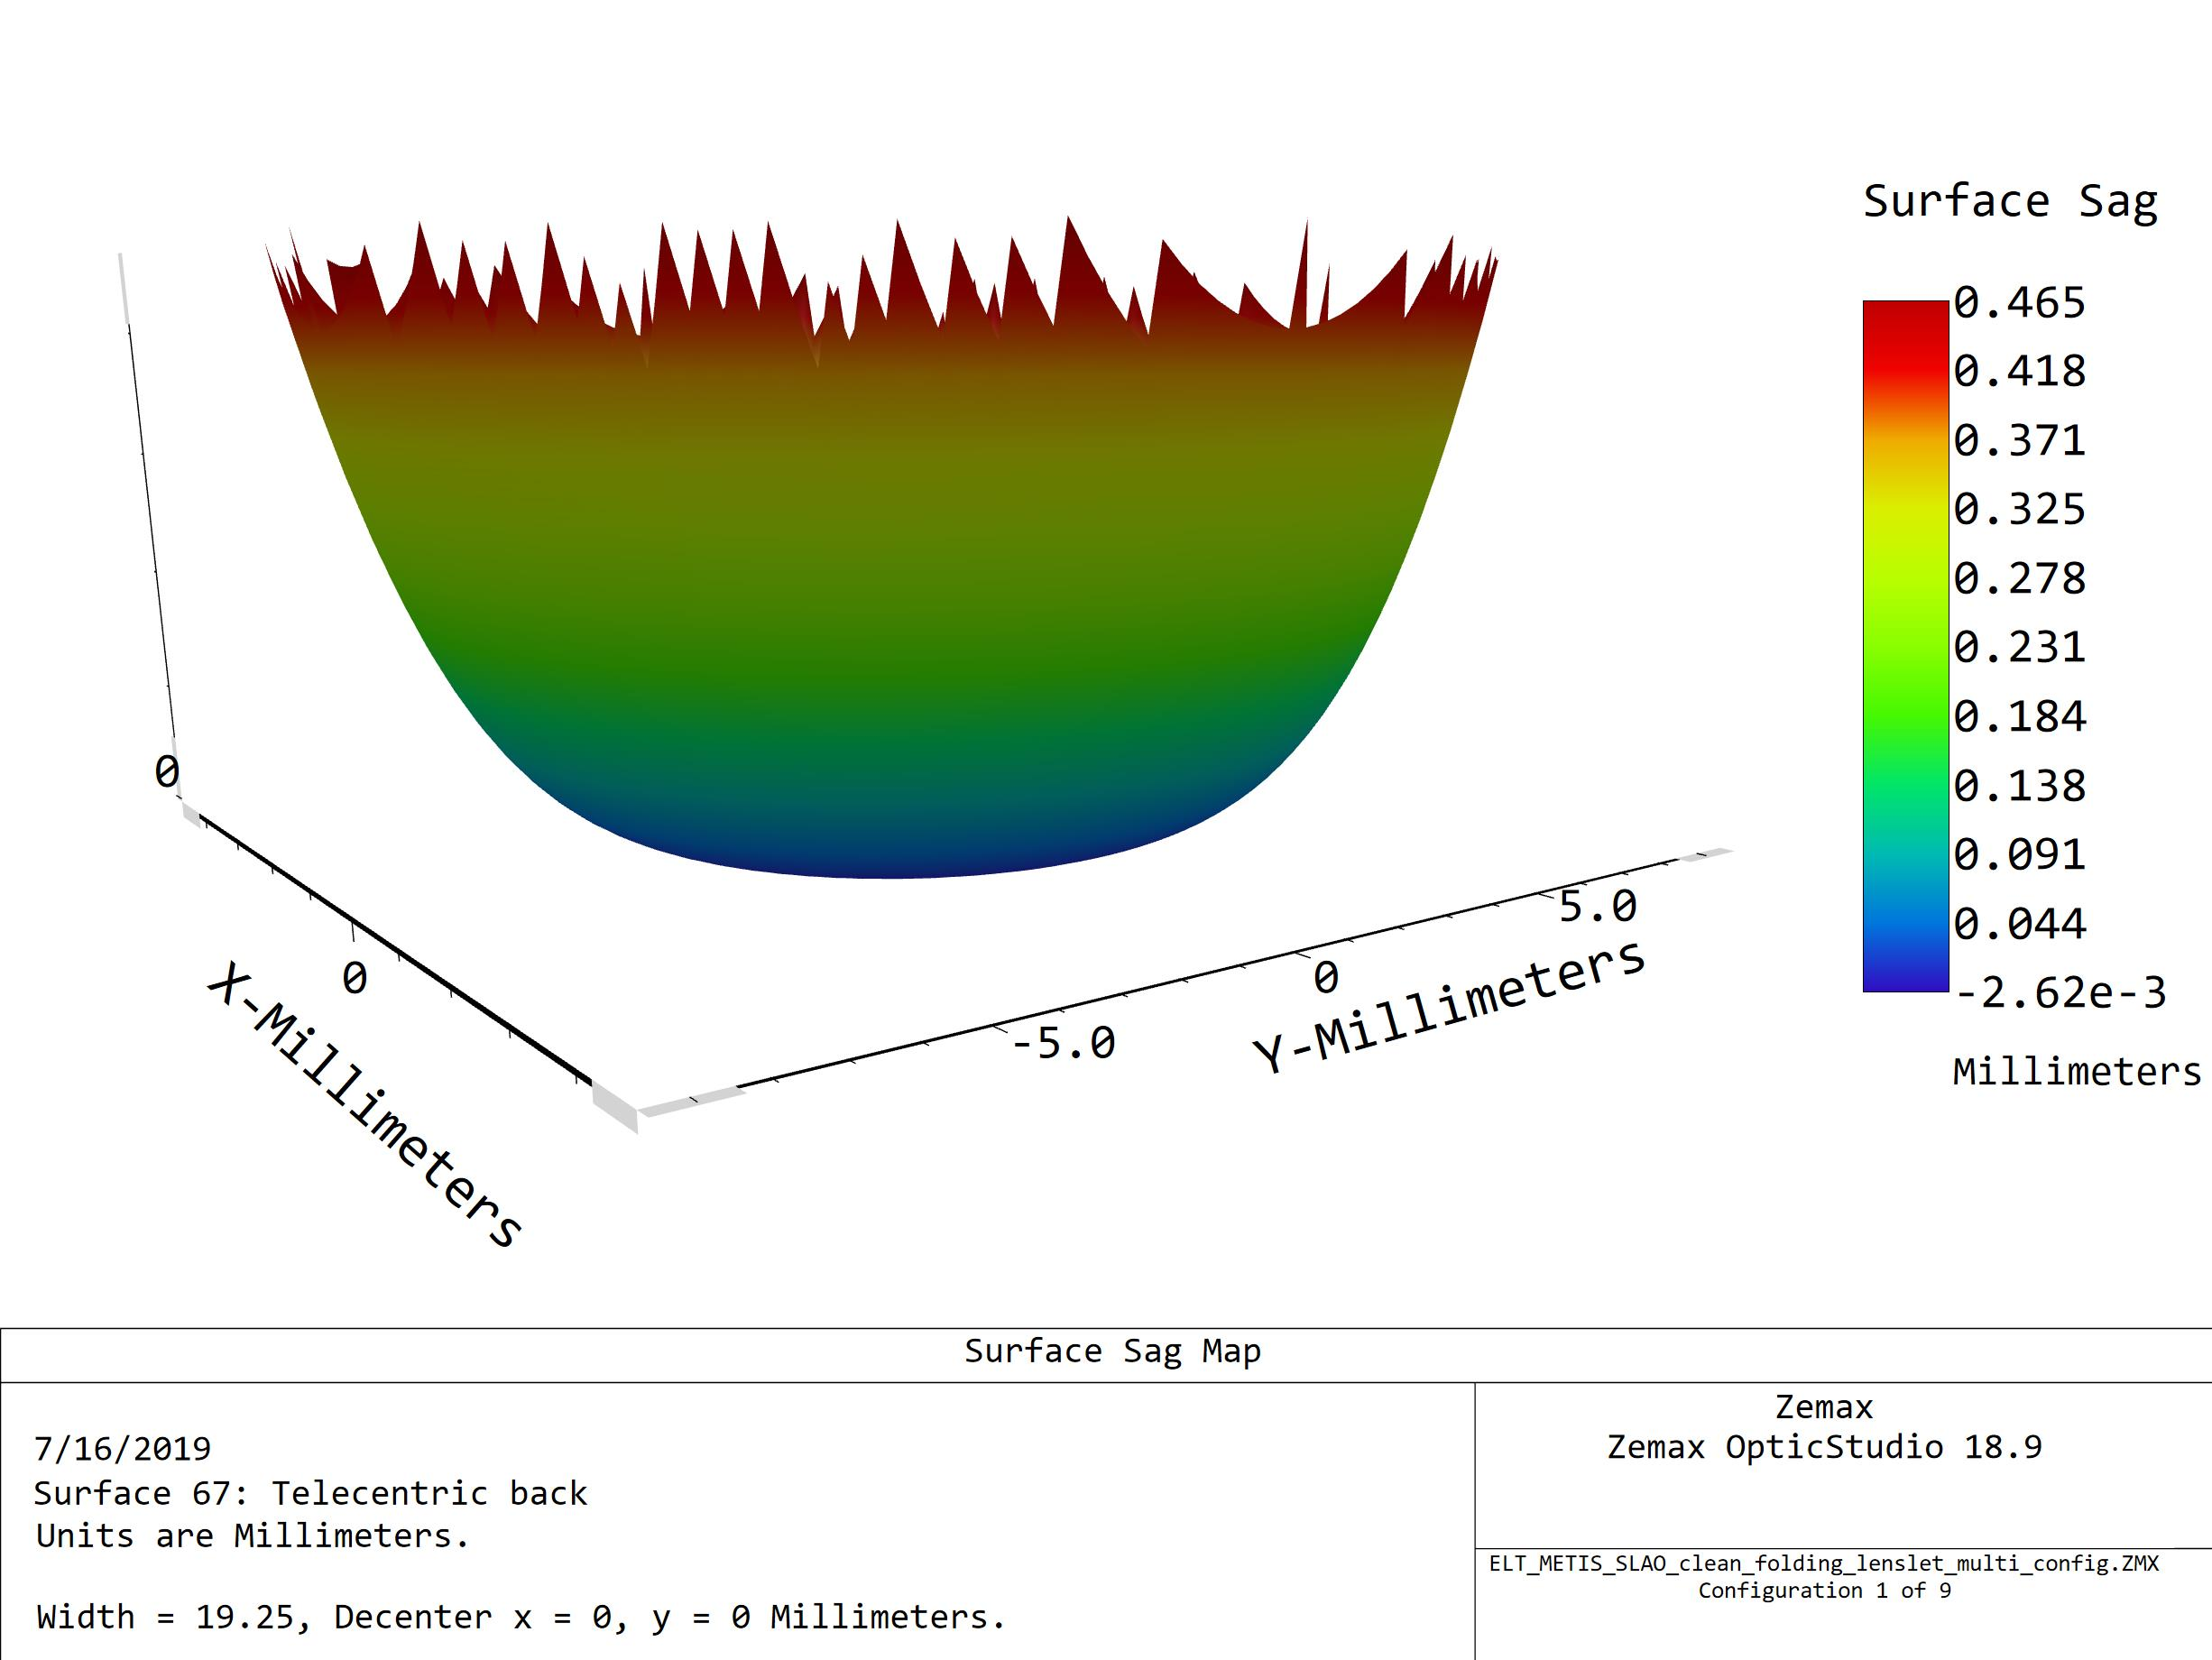
\includegraphics[width=14 cm]{Figures/SurfaceSag.jpg}
\caption{A Figure showing a surface map of the aspherical component.}
\label{fig:surface_sag}
\end{figure}